\documentclass[11pt,a4paper]{article}

\usepackage[utf8]{inputenc}
\usepackage[T1]{fontenc}
\usepackage[margin=2.5cm]{geometry}
\usepackage{amsmath,amssymb,amsthm}
\usepackage{booktabs}
\usepackage{array}
\usepackage{xcolor}
\usepackage{tikz}
\usetikzlibrary{arrows.meta,positioning,calc}
\usepackage{hyperref}
\setlength{\emergencystretch}{3em}
\sloppy

% ---------------------------------------------------------------------------
% Notation macros
% ---------------------------------------------------------------------------
\newcommand{\Jset}{\mathcal{J}}
\newcommand{\Mset}{\mathcal{M}}
\newcommand{\Eset}{\mathcal{E}}
\newcommand{\cat}{\,\Vert\,}
\newcommand{\R}{\mathbb{R}}
\newcommand{\code}[1]{\texttt{#1}}

\theoremstyle{remark}
\newtheorem*{remark}{Remark}

\title{The Job--Machine Edge Design (\code{jm\_design})\\
of the BOPO Actor for the Flexible Job Shop Problem}
\author{Mariana Correia}
\date{\today}

\begin{document}
\maketitle

\begin{abstract}
The \code{jm\_design} parameter controls how the job--machine \emph{action edges}
of the heterogeneous scheduling graph are built and how the actor scores them.
It accepts four values, \code{auto}, \code{baseline}, \code{edges} and \code{attn}
(\code{JM\_DESIGN\_CHOICES} in \code{src/train.py}). This document describes the
role of the action edges in the decision process, the three
defects of the original (\code{baseline}) design, how \code{edges} removes them on
the environment side, how \code{attn} also changes the scoring function of the
actor, and what each choice means for the trained model.
\end{abstract}

\tableofcontents

% ===========================================================================
\section{Context: where the action edges live}
\label{sec:context}

\subsection{The state graph}
At every decision step the environment (\code{FJSSPEnv}, \code{src/env.py})
represents the partial schedule as a heterogeneous graph with three node types:
\emph{operation}, \emph{job} and \emph{machine}. Let $\Jset$ be the set of jobs and
$\Mset$ the set of machines. For each job $j$ let $o_j$ denote its \emph{current}
operation, i.e.\ the first operation of $j$ that has not yet been scheduled, and let
$p_{j,m}>0$ be its processing time on an eligible machine $m$.

Among the edge types of the graph, one is special:
\[
  \Eset_{\mathrm{act}} = \{\, (m \to j) \;:\; j \text{ unfinished},\; p_{j,m} > 0 \,\}
  \qquad \text{type } (\code{machine},\code{exec},\code{job}).
\]
Every edge $(m\to j)\in\Eset_{\mathrm{act}}$ is a \emph{candidate action}:
``schedule the current operation of job $j$ on machine $m$''. Each such edge carries a
feature vector $e_{mj}\in\R^{5}$ (six columns in the batching~v2 representations, see
Section~\ref{sec:batching}). The \code{jm\_design} parameter only concerns this edge
type, its reverse, and the head that scores it.

\subsection{From graph to decision}
One decision follows the same pipeline under every design:
\begin{enumerate}
  \item \textbf{Mask.} \code{calculate\_mask()} builds the matrix of earliest start
        times $S\in\R^{|\Jset|\times|\Mset|}$ (\code{job\_start\_machines}) and the
        current processing times $P$ (\code{current\_job\_proc}). With
        \code{mask\_option}$=0$ it ranks by start time $S_{j,m}$; otherwise by earliest
        completion time (ECT) $C_{j,m}=S_{j,m}+P_{j,m}$. For every job, only the
        \code{sel\_k} best machines stay unmasked.
  \item \textbf{Normalisation.} \code{normalize\_state()} min--max scales every
        node-feature column and every edge-feature column to $[-1,1]$
        \emph{independently per column}, over the current graph.
  \item \textbf{Message passing.} A GNN (GATv2, GINE or TransformerConv), converted
        to a heterogeneous model by \code{to\_hetero}, computes node embeddings
        $h_v\in\R^{32}$. \code{to\_hetero} creates one copy of the convolution for each
        edge type and averages (\code{aggr='mean'}) the outputs of all relations that
        point into the same node type.
  \item \textbf{Scoring.} \code{ActorModel.forward} gives each action edge a scalar
        logit $s_{mj}$. Masked edges get $-\infty$, a softmax turns the logits into a
        categorical distribution, and one edge is sampled (training) or the argmax
        is taken (greedy evaluation).
  \item \textbf{Transition.} \code{step()} schedules the chosen pair, updates $S$, $P$
        and the machine free times, removes the scheduled job's action edges, adds
        new action edges for its next operation, and calls \code{calculate\_mask()}
        again.
\end{enumerate}
The feature vector $e_{mj}$ is therefore used in two places: inside message passing
(the GNN's edge attention / edge MLP has \code{edge\_dim}$=5$ inputs) and directly in the
score $s_{mj}$. The quality of $e_{mj}$ matters a lot.

% ===========================================================================
\section{The four values}
\label{sec:values}

\begin{center}
\begin{tabular}{>{\ttfamily}l p{11.5cm}}
\toprule
\normalfont\textbf{Value} & \textbf{Meaning} \\
\midrule
auto     & Not a design. Resolved at the start of \code{train()} by
           \code{resolve\_jm\_design}: \code{edges} for every representation built
           on \code{ojm} (\code{ojm} and all \code{ojmb\_*}), \code{baseline} for
           \code{oo} and \code{om}. Default of \code{main.py} and \code{param.py}. \\
baseline & The original design: action edges in one direction only, with features
           written once and never updated. \\
edges    & Environment-side fix: reverse edge type added and every action edge
           recomputed after each decision with one fixed column layout. \\
attn     & The environment of \code{edges}, plus a bilinear (attention-style)
           term in the actor's scoring head. \\
\bottomrule
\end{tabular}
\end{center}

Only representations built on \code{ojm} have job nodes linked to machines. Asking for
\code{edges} or \code{attn} with \code{oo}/\code{om} raises a \code{ValueError}.
Note that \code{run\_diagnostic\_job.py} defaults to \code{baseline} (not \code{auto}).
This is why the batching sweeps pass \code{--jm-design edges} explicitly.

% ===========================================================================
\section{The \texttt{baseline} design and its three defects}
\label{sec:baseline}

\subsection{How the features are produced}
Under \code{baseline} the action-edge features are written \emph{once}, at the moment the edge
is created, and there are two different places that create edges:

\paragraph{In \code{reset()}} (first operation of every job; every machine is free and
every job is ready at time $0$):
\[
  e^{\mathrm{reset}}_{mj} =
  \Bigl[\; p_{j,m},\;\; \tfrac{p_{j,m}}{\sum_{m'} p_{j,m'}},\;\;
        \tfrac{p_{j,m}}{\sum_{m'} p_{j,m'}},\;\; 0,\;\; p_{j,m} \;\Bigr].
\]

\paragraph{In \code{step()}} (next operation of the job just scheduled). Let $E_j$ be the
end time of job $j$'s previous operation, $F_m$ the time machine $m$ becomes free, and
$g_{j,m}=p_{j,m}+\max(E_j-F_m,0)$:
\[
  e^{\mathrm{step}}_{mj} =
  \Bigl[\; g_{j,m},\;\; \tfrac{p_{j,m}}{\sum_{m'} p_{j,m'}},\;\;
        p_{j,m}+\max(E_j,F_m),\;\; \tfrac{g_{j,m}}{\sum_{m'} g_{j,m'}},\;\; 0 \;\Bigr].
\]

\subsection{Defect 1: stale features}
After an action $(m^\star, j^\star)$ with completion time $c^\star$, the environment updates
\[
  S_{j,m^\star} \leftarrow \max(S_{j,m^\star},\, c^\star) \qquad \forall j,
\]
so the mask immediately knows that every other job waiting for $m^\star$ now starts later.
The edge features of those jobs, however, are \emph{not} touched. The network
sees the old start/completion values, while the mask uses the new ones. The two
contradict each other, and the further the episode goes, the larger the error.

\subsection{Defect 2: inconsistent column semantics}
Comparing $e^{\mathrm{reset}}$ and $e^{\mathrm{step}}$ column by column:

\begin{center}
\begin{tabular}{c l l}
\toprule
Col. & Edge created in \code{reset()} & Edge created in \code{step()} \\
\midrule
0 & processing time $p$            & processing time + job wait $g$ \\
1 & relative processing time       & relative processing time \\
2 & relative processing time (dup.)& completion time \\
3 & $0$                            & relative $g$ \\
4 & processing time $p$            & $0$ \\
\bottomrule
\end{tabular}
\end{center}

Only column~1 means the same thing in both. The same weight of the network multiplies
a ratio for some edges and an absolute time for others, and the column-wise normalisation
mixes the two populations. A linear layer cannot learn one consistent use of a column
whose meaning depends on when the edge was created.

\subsection{Defect 3: one-directional information flow}
Only $(m\to j)$ edges exist. A job receives messages from the machines that can process it,
but a machine receives nothing from the jobs that compete for it. Its embedding is built
only from the operation--machine relation, so it cannot directly encode ``three urgent jobs
are waiting for me''.

\subsection{A worked example}
\label{sec:example}
Two machines $M_1,M_2$, two jobs at their first operation:
$p_{1,1}=4$, $p_{1,2}=6$ (job $J_1$ is eligible on both) and $p_{2,1}=3$ ($J_2$ only on $M_1$).
Use ECT masking with \code{sel\_k}$=1$.

At reset all starts are $0$. The policy schedules $J_2$ on $M_1$, so $M_1$ is busy until $3$ and
$S_{1,1}\leftarrow 3$. For $J_1$ the mask now compares $C_{1,1}=3+4=7$ with $C_{1,2}=0+6=6$,
and keeps $M_2$.

\begin{center}
\begin{tabular}{l c c}
\toprule
 & edge $M_1\to J_1$ & edge $M_2\to J_1$ \\
\midrule
\code{baseline} (unchanged since reset) & $[4,\,0.4,\,0.4,\,0,\,4]$ & $[6,\,0.6,\,0.6,\,0,\,6]$ \\
\code{edges} (refreshed)               & $[4,\,0.4,\,3,\,7,\,0]$   & $[6,\,0.6,\,0,\,6,\,0]$ \\
\bottomrule
\end{tabular}
\end{center}

Under \code{baseline}, the network's features say $M_1$ is the better machine for $J_1$
(shorter processing, nothing about the delay), while the mask has already decided that
$M_2$ is better. Under \code{edges}, column~3 holds exactly the value the mask ranks, and
the conflict disappears.

% ===========================================================================
\section{The \texttt{edges} design}
\label{sec:edges}

\code{edges} changes \emph{only the environment}. The actor's architecture is the
same as in \code{baseline}, except that the GNN gets one more relation to process.

\subsection{Recomputing every action edge after each decision}
At the end of every \code{calculate\_mask()} call (in \code{reset()} and after every
\code{step()}), \code{\_refresh\_jm\_edges()} overwrites the features of \emph{all} action
edges, masked or not, from the same live matrices the mask uses. With $S_{j,m}$ the earliest
start, $P_{j,m}=p_{j,m}$ the current processing time and $F_m$ the machine free time
(machine feature~0):
\[
  e_{mj} =
  \Bigl[\;
    \underbrace{P_{j,m}}_{\text{0: proc.\ time}},\;\;
    \underbrace{\tfrac{P_{j,m}}{\sum_{m'}P_{j,m'}}}_{\text{1: relative speed}},\;\;
    \underbrace{S_{j,m}}_{\text{2: start}},\;\;
    \underbrace{S_{j,m}+P_{j,m}}_{\text{3: completion (ECT)}},\;\;
    \underbrace{\max(S_{j,m}-F_m,\,0)}_{\text{4: idle created}}
  \;\Bigr].
\]
\begin{itemize}
  \item \textbf{Column 0} is the cost of the operation on $m$.
  \item \textbf{Column 1} compares $m$ with the other eligible machines. A small value
        means $m$ is a fast choice for this operation.
  \item \textbf{Column 2} is the earliest time the operation can start on $m$:
        $S_{j,m}=\max(E_j,F_m)$, kept up to date as other jobs occupy $m$.
  \item \textbf{Column 3} is the earliest completion time, the very quantity the ECT mask
        and the warm-start teacher rank by.
  \item \textbf{Column 4} is the gap the machine would sit idle waiting for job $j$
        to become ready ($E_j>F_m$). It is a direct signal of wasted capacity.
\end{itemize}
All five columns mean the same thing for every edge at every step, which fixes Defects
1 and 2.

\subsection{The reverse edge type}
The same function also writes
\[
  (\code{job},\code{exec},\code{machine}):\quad
  \text{edge\_index} = \text{flip}(\text{edge\_index}_{\mathrm{act}}),\qquad
  e_{jm} = e_{mj}.
\]
This mirrored relation is used only for message passing; actions are still taken on the
$(m\to j)$ edges. Because \code{to\_hetero} builds one convolution per relation, the
machine embedding becomes
\[
  h_m^{(\ell+1)} = \tfrac12\Bigl(
     \mathrm{Conv}^{(\ell)}_{\mathrm{op}\to m}\bigl(h^{(\ell)}\bigr) +
     \mathrm{Conv}^{(\ell)}_{j\to m}\bigl(h^{(\ell)}, e\bigr)
  \Bigr),
\]
so every machine now aggregates the jobs that compete for it, weighted by the
start/completion/idle values of those candidate assignments (Defect 3). With $L$ layers,
information can also flow job $\to$ machine $\to$ job: a job can ``see'' its competitors
through a shared machine.

The reverse edge type is also included in the per-column normalisation of
\code{normalize\_state()}.

\begin{figure}[ht]
\centering
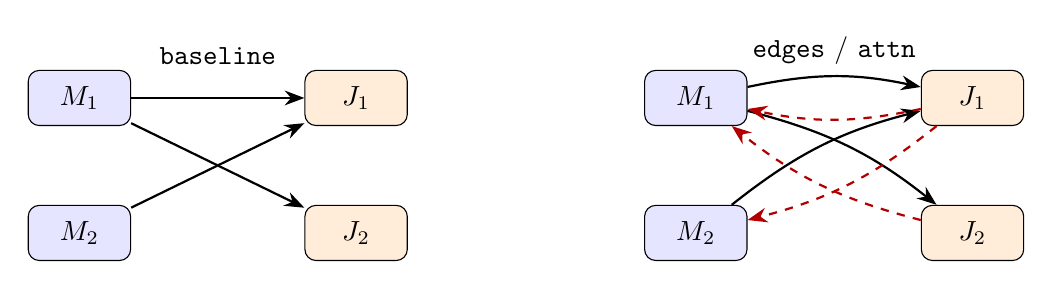
\begin{tikzpicture}[
  node distance=1.0cm and 2.2cm,
  mach/.style={draw, rounded corners, fill=blue!10, minimum width=1.3cm, minimum height=0.7cm},
  jobn/.style={draw, rounded corners, fill=orange!15, minimum width=1.3cm, minimum height=0.7cm},
  act/.style={-{Stealth[length=2.5mm]}, thick},
  rev/.style={-{Stealth[length=2.5mm]}, thick, dashed, red!70!black}]
  % baseline
  \node[mach] (m1) {$M_1$};
  \node[mach, below=of m1] (m2) {$M_2$};
  \node[jobn, right=of m1] (j1) {$J_1$};
  \node[jobn, right=of m2] (j2) {$J_2$};
  \draw[act] (m1) -- (j1);
  \draw[act] (m2) -- (j1);
  \draw[act] (m1) -- (j2);
  \node[above=0.3cm of $(m1)!0.5!(j1)$] {\code{baseline}};
  % edges
  \node[mach, right=3.0cm of j1] (n1) {$M_1$};
  \node[mach, below=of n1] (n2) {$M_2$};
  \node[jobn, right=of n1] (k1) {$J_1$};
  \node[jobn, right=of n2] (k2) {$J_2$};
  \draw[act] (n1) to[bend left=12] (k1);
  \draw[act] (n2) to[bend left=12] (k1);
  \draw[act] (n1) to[bend left=12] (k2);
  \draw[rev] (k1) to[bend left=12] (n1);
  \draw[rev] (k1) to[bend left=12] (n2);
  \draw[rev] (k2) to[bend left=12] (n1);
  \node[above=0.3cm of $(n1)!0.5!(k1)$] {\code{edges} / \code{attn}};
\end{tikzpicture}
\caption{Action edges (solid, scored by the actor) and the mirrored job$\to$machine
relation (dashed, message passing only) for the example of Section~\ref{sec:example}.}
\end{figure}

\subsection{Effect on the warm-start teacher}
Before BOPO starts, the policy is pre-trained by behaviour cloning on
\code{expert\_action()}. Among the unmasked candidates, this rule picks the smallest
mask criterion and breaks ties with the other time: start then completion for
\code{mask\_option}$=0$, completion then start otherwise. Ties happen often (71\% of
decisions with \code{mask\_option}$=0$). Both quantities are columns~2 and~3 of the
refreshed edges, so under \code{edges} the teacher's choice is a function of what the
network sees, and it can be imitated. Under \code{baseline} the network sees neither
quantity correctly, and the teacher is much harder to fit.

% ===========================================================================
\section{The \texttt{attn} design}
\label{sec:attn}

The environment is identical to \code{edges}: \code{FJSSPEnv} treats
\code{"edges"} and \code{"attn"} the same way. The difference is in
\code{ActorModel}.

\subsection{Limitation of the linear head}
Under \code{baseline} and \code{edges} the logit of an action is
\[
  s_{mj} = w^\top\bigl[\,h_m \cat e_{mj} \cat h_j\,\bigr] + b
         = a^\top h_m + c^\top e_{mj} + d^\top h_j + b .
\]
This is \emph{additive} in the machine and the job. For a fixed job $j$, the term
$d^\top h_j$ is the same for every machine. The ranking of $j$'s machines therefore depends
only on $a^\top h_m + c^\top e_{mj}$: the job's own embedding cannot change \emph{which}
machine is preferred for it. The head cannot express ``this job fits this
machine'', only ``this job is generally urgent'' plus ``this machine is generally good''.
Any job--machine interaction has to be packed into $e_{mj}$ or created indirectly
by message passing.

\subsection{The bilinear term}
With \code{attn}, three extra linear maps $W_q, W_k, W_e$ (output dimension $d=64$)
are created, and the logit becomes
\[
  s_{mj} = \underbrace{w^\top\bigl[\,h_m \cat e_{mj} \cat h_j\,\bigr] + b}_{\text{linear head, as before}}
  \;+\;
  \frac{\bigl(W_q h_j\bigr)^{\!\top}\bigl(W_k h_m + W_e e_{mj}\bigr)}{\sqrt{d}} .
\]
This is the same form TransformerConv uses for its attention logits: the job acts as
the \emph{query}, the machine (corrected by the edge features) as the \emph{key}. The
product $h_j^\top W_q^\top W_k h_m$ is a learned similarity between the two embeddings,
so the preferred machine can now differ from job to job. The term
$h_j^\top W_q^\top W_e e_{mj}$ lets each job weight the edge features differently
(for example, one job cares about idle time, another about completion time). The factor
$1/\sqrt{d}$ keeps the variance of the dot product comparable to the linear term at
initialisation.

\begin{remark}
The extra layers are created only when \code{jm\_design="attn"}. \code{baseline} and
\code{edges} therefore build exactly the same parameters, and use the random number
generator the same way, as before the option existed. Runs with the same seed
stay comparable.
\end{remark}

% ===========================================================================
\section{Interaction with the batching representations}
\label{sec:batching}

The batching environments (\code{src/env\_batching.py}) override
\code{\_refresh\_jm\_edges()} on top of the base version:
\begin{itemize}
  \item For the \emph{node} and \emph{edge} batching representations, columns~0 and~3 hold
        the processing and completion time of the \emph{batch} the action would dispatch
        (its longest member), since that is what the action really costs. The
        \emph{base} representation keeps the individual operation's time, so its graph
        stays free of batching information.
  \item In batching~v2 a sixth column is appended: the number of operations the action
        dispatches (all zeros for \emph{base}, so that every v2 representation has the
        same width).
  \item Wait actions (``wait for a larger batch'') are extra action edges. Only when
        \code{jm\_design}$\neq$\code{baseline} are their columns~2--4 overwritten with
        the waiting start time $s_w$, completion $s_w+p$ and idle time $s_w-F_m$. Under
        \code{baseline} they would keep the values of the non-waiting action and look
        identical to it.
  \item After any edge is added or removed, \code{\_sync\_reverse\_edges()} mirrors the
        action edges onto the job$\to$machine relation again.
\end{itemize}
In short, the batching information is carried mainly by the refreshed action edges. The
batching experiments are only meaningful with \code{edges} (or \code{attn}), which is
why all of them use \code{edges}.

% ===========================================================================
\section{Consequences for the trained model}
\label{sec:consequences}

\begin{center}
\begin{tabular}{l p{3.3cm} p{3.4cm} p{3.4cm}}
\toprule
 & \code{baseline} & \code{edges} & \code{attn} \\
\midrule
Relations seen by GNN & machine$\to$job only & + job$\to$machine & + job$\to$machine \\
Edge features & stale, two layouts & refreshed each step, one layout & refreshed each step, one layout \\
Scoring head & linear & linear & linear + bilinear \\
Extra parameters & --- & one conv per layer for the new relation & same as \code{edges} + $W_q,W_k,W_e$ \\
Env.\ cost per step & lowest & one vectorised refresh & same as \code{edges} \\
\bottomrule
\end{tabular}
\end{center}

\begin{enumerate}
  \item \textbf{The architecture depends on the design.} The graph metadata passed to
        \code{to\_hetero} is read from the first state of the environment
        (\code{s.metadata()} in \code{train()}). Under \code{edges}/\code{attn} that state
        already contains the reverse relation, so the model has more convolution
        weights. Under \code{attn} it also has the three attention maps.
  \item \textbf{Checkpoints are tied to their design.} A model trained with one value cannot
        be loaded or evaluated with another. For this reason \code{jm\_design} is
        stored in \code{model\_params}, and \code{run\_metrics.py},
        \code{rescore\_checkpoints.py} and the test code in \code{train.py} read it back
        and rebuild the environment with the same value. Old entries without
        the key are treated as \code{baseline}.
  \item \textbf{The features and the mask agree.} With \code{edges}, the policy sees the
        quantities that decide whether an action is unmasked and how it ranks. Learning then
        focuses on choosing \emph{among} the good candidates, instead of first
        working out a criterion from features that contradict it.
  \item \textbf{Comparability.} Comparisons between representations or GNN types should
        keep \code{jm\_design} fixed. Changing it changes both the input
        and the architecture.
\end{enumerate}

% ===========================================================================
\section{Usage}

\begin{verbatim}
# default: auto -> edges for ojm / ojmb_*, baseline for oo / om
python main.py --representation ojm

# explicit choice
python main.py --representation ojm --jm-design baseline
python main.py --representation ojm --gnn-type transformer --jm-design attn

# diagnostic / batching runs (default there is baseline, so set it)
python run_diagnostic_job.py --representation ojmb_node --jm-design edges ...
\end{verbatim}

The resolved value is printed at the start of every run:
\begin{verbatim}
[TRAIN] Representation | ojmb_node_v2 | GNN | gat | jm_design | edges
\end{verbatim}

% ===========================================================================
\section{Summary}
\begin{itemize}
  \item \code{auto} picks \code{edges} whenever job--machine edges exist, and
        \code{baseline} otherwise.
  \item \code{baseline}: action-edge features are written once, become stale as the schedule
        progresses, mean different things depending on where they were created, and flow
        in one direction only.
  \item \code{edges}: every action edge is recomputed after each decision with
        $[\,p,\; p/\!\sum p,\; S,\; S+p,\; \text{idle}\,]$, and mirrored onto a
        job$\to$machine relation, so machines see their competing jobs.
  \item \code{attn}: \code{edges} plus a query--key term
        $(W_q h_j)^\top(W_k h_m + W_e e_{mj})/\sqrt{d}$ that lets the actor score how well a
        specific job matches a specific machine.
\end{itemize}

\end{document}
